\subsection{Существование нестандартных моделей арифметики. Теорема о порядке на галактиках в этих моделях}

Здесь собрана информация их разных источников. Однако есть лекция Мусотова на эту тему. Там разбирают тему билета.

\href{https://mipt.lectoriy.ru/lecture/Maths-MathemLogic-L15-Musatov-141210.01}{ссылка: лекция Мусотова}

\textbf{Нестандартные модели арифметики}

\textbf{Пример.} Пусть $(\mathbb{N}; =, S, +, \cdot, 0)$ — стандартная модель арифметики и $Th(\mathbb{N})$
есть множество всех истинных в $\mathbb{N}$ предложений (теорий).

Добавим к сигнатуре новую константу $\Omega$ и рассмотрим теорию
$$T \rightleftharpoons Th(\mathbb{N}) \cap \{\neg \Omega = 0, \neg \Omega = S0, \neg \Omega = SS0, \ldots \}$$
или аналогичную
$$T \rightleftharpoons Th(\mathbb{N}) \cap \{\Omega > 0, \Omega > 1, \Omega > 2, \ldots \}$$

$T$ — тоже теория, и к ней также применима теорема о компактности. У такой теории любая конечная подтеория — совместна. Из теоремы о компактности следует, что у данной теории существует модель, то есть вся теория — совместна. Эта модель арифметики уже не может быть стандартной.
Значит, она должна заключать в себе стандартную модель.

\textbf{Определение.} Терм $\bar n \rightleftharpoons SS \ldots S0$ ($n$ раз) называем \textit{нумералом}. Нумералы служат именами натуральных чисел.

\textbf{Определение.} Введем обозначение $^*N$ это носитель новой модели, а ее элементы будем называть \textit{гипернатуральными числами}. Будем изучать такую модель. Заметим, что здесь $\Omega$ — это
«бесконечно большое число».

\textbf{Корректность:}
Здесь существует операция прибавления единицы $(Sx = x + 1)$. Значит, функция всюду определена. Тогда применим ее к $\Omega$:
$$S \Omega = \Omega + 1 > \Omega.$$

Отношение порядка:
$$\forall x \not \exists y \ \ \ x < y < x + 1.$$
Можно также записать:
$$S(\Omega + 1) = \Omega + 2, S(\Omega + 2) = \Omega + 3, \ldots .$$
Так будет построено счетное количество, которое, с точки зрения порядка, образует внутри себя натуральный ряд. Также из любого числа, кроме нуля, можно вычесть единицу:
$$\forall x (x \neq 0 \rightarrow \exists y \ s(y) = x)$$.
Обозначим также:
$$\Omega = S(\Omega - 1).$$
Если считать, что вычитание — это частично определенная функция, то это будет не только обозначение, но и содержательное утверждение.
Аналогично:
$$\Omega - 1 = S(\Omega - 2), \ldots$$
С точки зрения порядка получим некий аналог целых чисел. Более того, такие утверждения можно провести не только с $\Omega$, но и с любыми нестандартным числом.
Заметим, что любое нестандартное число должно быть больше любого стандартного

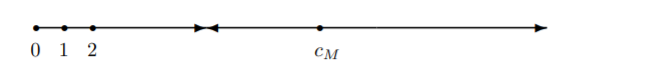
\includegraphics[scale=1]{images/1.16_стрелка1.PNG}

(картинка не совсем верная: $\mathbb{N}$ и галактика, порождённая $c_M = \Omega$, не находятся вплотную)

Два варианта доказательства существования нестандартных моделей арифметики. Выбирайте удобный:

\textbf{Существование. 1-ый вариант доказательства.} (Из теоремы компактности)

Существование нестандартных моделей арифметики может быть продемонстрировано применением теорема компактности. Для этого набор аксиом $T$ определяется на языке, включающем язык арифметики Пеано, вместе с новым постоянным символом $\Omega$. Аксиомы состоят из аксиом арифметики Пеано $Th(\mathbb{N})$ вместе с другим бесконечным набором аксиом: для каждого числа $n$ аксиома $\Omega > n$ включена. $T \rightleftharpoons Th(\mathbb{N}) \cap \{\Omega > 0, \Omega > 1, \Omega > 2, \ldots \}$ Любое конечное подмножество этих аксиом удовлетворяется моделью, которая представляет собой стандартную модель арифметики. Константа $\Omega$ интерпретируется как некоторое число больше любого числа, упомянутого в конечном подмножестве $T$. Таким образом, по теореме компактности существует модель, удовлетворяющая всем аксиомам $T$. Поскольку любая модель $T$ является моделью $Th(\mathbb{N})$ (поскольку модель набора аксиом, очевидно, также является моделью любого подмножества этого набора аксиом), мы имеем, что наша расширенная модель также является моделью аксиом Пеано. Элемент этой модели, соответствующий $\Omega$ не может быть стандартным числом, потому что, как указано, оно больше любого стандартного числа.

\textbf{Существование. 2-ой вариант доказательства.} (Из теоремы компактности)

$T \rightleftharpoons Th(\mathbb{N}) \cap \{\Omega > 0, \Omega > 1, \Omega > 2, \ldots \}$

По теореме о компактности (видимо исчисления предикатов) существует (нормальная) модель $M \vDash T$. Модель $M$ обладает следующими свойствами:
\begin{itemize}
\item $\mathbb{N}$ изоморфна начальному сегменту $M$; вложение $\mathbb{N} \rightarrow M$ задаётся функцией $\phi : n \rightarrow \bar n_M$.

\item $M \vDash Th(\mathbb{N})$ ($M$ - модель множества $Th(\mathbb{N})$)

\item Бывает что $M \not \cong \mathbb{N}$, а бывает $M \not \cong \mathbb{N}$, в частности $\Omega \in M$ есть «бесконечно большое число», поскольку $\Omega$ отлично от всякого $n \in \mathbb{N}$.

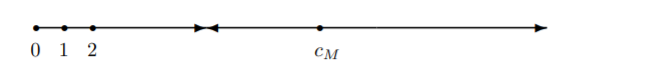
\includegraphics[scale=1]{images/1.16_стрелка1.PNG}

Формула $a < b \rightleftharpoons \exists x(x \neq 0 \wedge a + x = b)$ определяет порядок в $\mathbb{N}$. Для данной формулы в $\mathbb{N}$ выполнены аксиомы строгого линейного порядка и следующие
предложения:
\item $\forall x (0 < x \vee 0 = x)$;
\item $\forall x\exists y (x < y \wedge \forall z (z < y \rightarrow  z = x \vee z < x))$;
\item $\forall y (y \neq 0 \rightarrow  \exists x (x < y \wedge \forall z (z < y \rightarrow  z = x \vee z < x)))$.
\end{itemize}

Следовательно, те же аксиомы выполнены и в $T$. Поэтому предикат $<_T$ на $T$ представляет собой строгий линейный порядок с наименьшим элементом $0$. При этом каждый элемент имеет последователя, и каждый элемент, кроме $0$, имеет непосредственного предшественника.

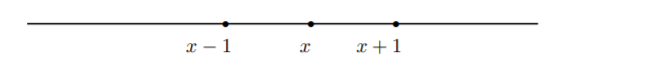
\includegraphics[scale=1]{images/1.16_стрелка2.PNG}

\textbf{Определение.} Элементы $x, y \in  M$ близки, если для некоторого $n \in  \mathbb{N}$ выполнено $y = SS \ldots S(x)$ или $x = SS \ldots S(y)$ ($n$ символов $S$).
Классы эквивалентности по отношению близости называем \textbf{галактиками}.

\textbf{Определение.} (аналогичное) С любым нестандартным числом $x$ связано множество следующего вида:
$$\{\ldots , x - 2, x - 1, x , x  + 1, x + 2, \ldots \}.$$
Такое множество называется \textit{нестандартной галактикой}.

$\mathbb{N}$ - стандартная галактика.

\textbf{Утверждение.} Если $G$ — галактика в $M$, $G \neq \mathbb{N}$, то порядок $(G, <_M)$ изоморфен $(\mathbb{Z}, <)$.

Пусть $\mathcal{G}$ есть множество всех галактик в $M$. Определим $G_1 <_M G_2$, если для любых $x \in  G_1, y \in  G_2, x <_M y$.

\textbf{Утверждение.(на множестве галактик задан линейный порядок)} Если $G$ и $H$ — две различные галактики в $M$, и для некоторых $x_0 \in G$ и $y_0 \in H$ верно $x_0 < y_0$, тогда:
$$\forall x \in G \ \forall y \in H \ \ x < y.$$

$\blacktriangle$ Пусть:
$$x_0 + a \geq y_0 + b$$
Тогда можно записать:
$$-x_0 + y_0 > 0, \ \ x_0 - y_0 - b + a \geq 0.$$
Соответственно, в стандартной модели для $x_0$ и $y_0$ можно записать формулу, верную и в гипернатуральных числах.
Рассуждения приводят к противоречию по причине того, что $x_0$ и $y_0$ лежат в различных галактиках. Таким образом, доказано, что на множестве галактик задан линейный порядок. $\blacksquare$

\textbf{Утверждение. (б/д)} Любое нестандартное число больше любого стандартного. 

\textbf{Утверждение.} $\mathbb{N}$ - минимальный элемент $\mathcal{G}.$

$\blacktriangle$ Любая другая галактика $G$ в $\mathcal{G}$ является нестандартной. Сл-но, любой элемент $\mathbb{N}$ меньше любого элемента $G$. Сл-но, $\mathbb{N}$ - минимальный элемент $\mathcal{G}.$
$\blacksquare$

Так как в $T$ работают те же операции, что и в $Th(\mathbb{N})$, то в модели $M$ есть операции сложения, вычитания, умножения и деления (только аккуратные, чтобы число оставались натуральными илм гипернатуральными) на число из $\mathbb{N}$ (соответсвенно и на рациональные).

\textbf{Утверждение. (б/д)} У $\mathcal{G}$ нет наибольшего элемента.

$\blacktriangle$
Для натуральных чисел есть опперация $d(x) = 2x$. Для гипернатуральных чисел есть соответсвующая опперация $d(x) = 2x$. Могут ли $\Omega$ и $d(\Omega)$ лежать в одной галактике?

Так как для натуральных чисел выполняется $\forall x \ |d(x) - x| = x$, то и это выполняется для гипернатуральных. Сл-но, разность между $\Omega$ и $d(\Omega)$ это гипернатуральное число. Сл-но, они в разных галактиках.
$\blacksquare$

\textbf{Утверждение. (б/д)} Пусть $d_{\alpha}(x) = [\alpha x]$. Тогда, если $\alpha < \beta$, то $d_{\alpha}(x)$ и $d_{\beta}(x)$ в разных галактиках.

$\blacktriangle$
Доказывается аналогично: Разность $d_{\alpha}(x)$ и $d_{\beta}(x)$ это гипернатуральное число. Сл-но, они в разных галактиках:
$\exists N \forall x > N \ d_{\beta}(x) - d_{\alpha}(x) > d_{\frac{\alpha + \beta}{2}}(x)$
$\blacksquare$

\textbf{Утверждение.множество галактик имеет плотный порядок}
Если $G$ и $H$ — две различные галактики в $M$, и $G < H$, тогда:
$$\exists F \text{- галактика: } G < F < H$$

Доказывается аналогично. Это можно также показать, если аккуратно применить $c_{\alpha}(x, y) = [\alpha x + (1 - \alpha) y]$, где $x \in G, y \in H, \alpha \in (\mathbb{R} \geq 0)$. $c_{\alpha}(x, y)$ - галактика. Тогда порядок плотный, так как на $\mathbb{R}$ плотный порядок.